To house all the components that make the DSP, a 19 inch 2U rack case is used. These cases are used for a lot of audio processing devices. This makes it easier to keep a system organized. The DSP fits nicely into an existing audio rack somebody may use.
\par 
\noindent The case is fitted with all the needed ports on the back, a screen and knob in the front left, and 16 LEDs for showing VU-readings in the front right (not showed on CAD drawing). Power is connected via a metal female DC connector so that, when not in use, the case has no wires attached. 
\par
\noindent Mounted inside the case is an FPGA-board and a custom PCB loaded with all the needed converters. The FPGA-board and PCB are mounted on metal spacers connected to the case with screws. This way of mounting the components was chosen to have a sturdy, robust product.

\begin{figure}[ht]
    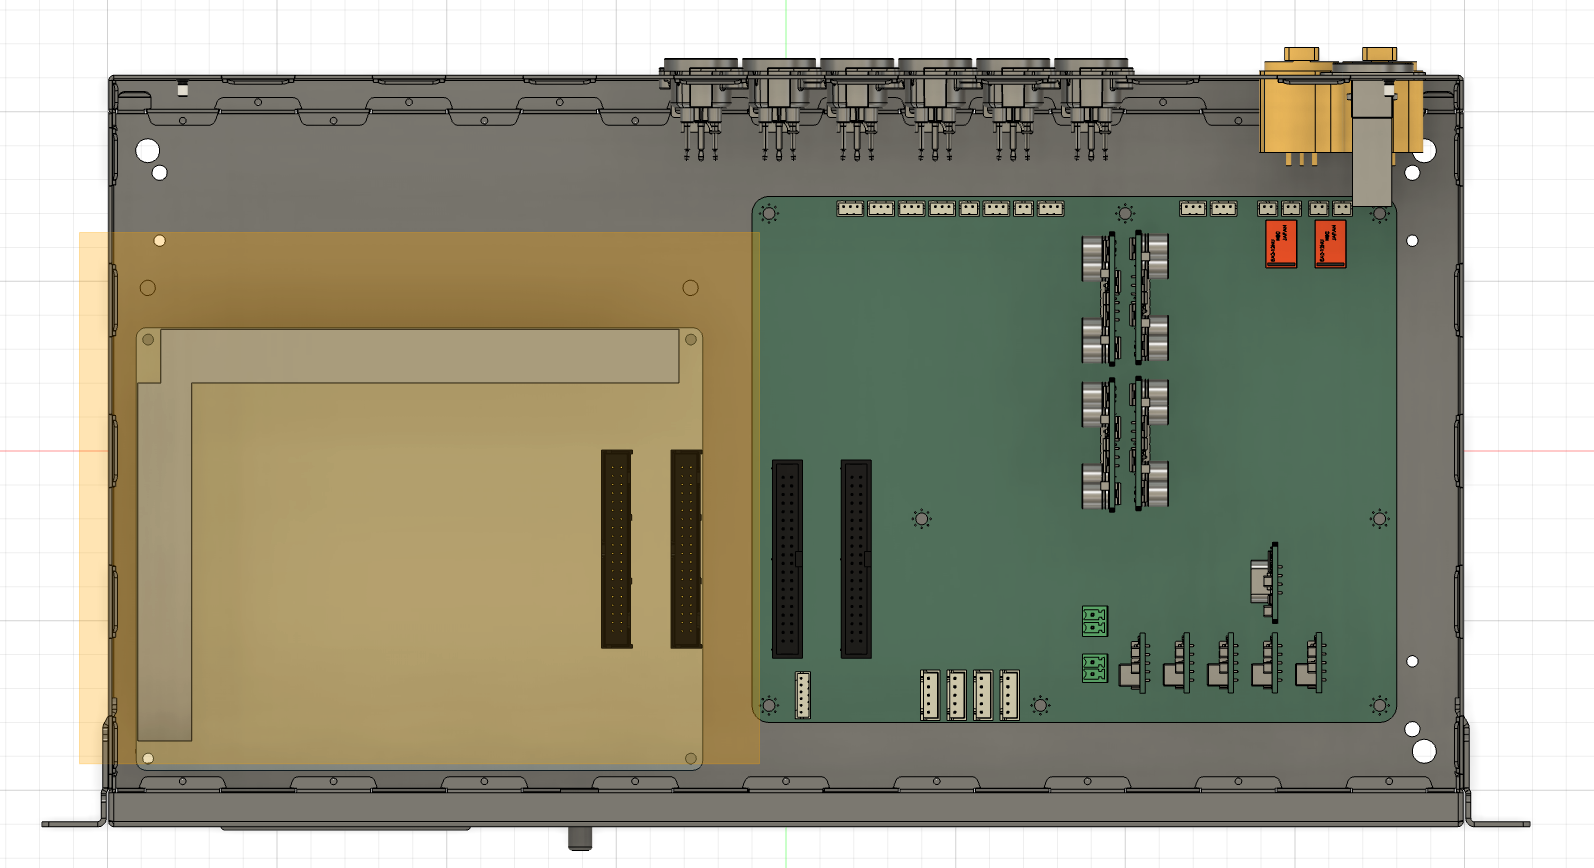
\includegraphics[width=0.8\textwidth]{topviewcase}
    \caption{Top-down view of the case}
    \label{fig:topview}
\end{figure}

\begin{figure}[ht]
    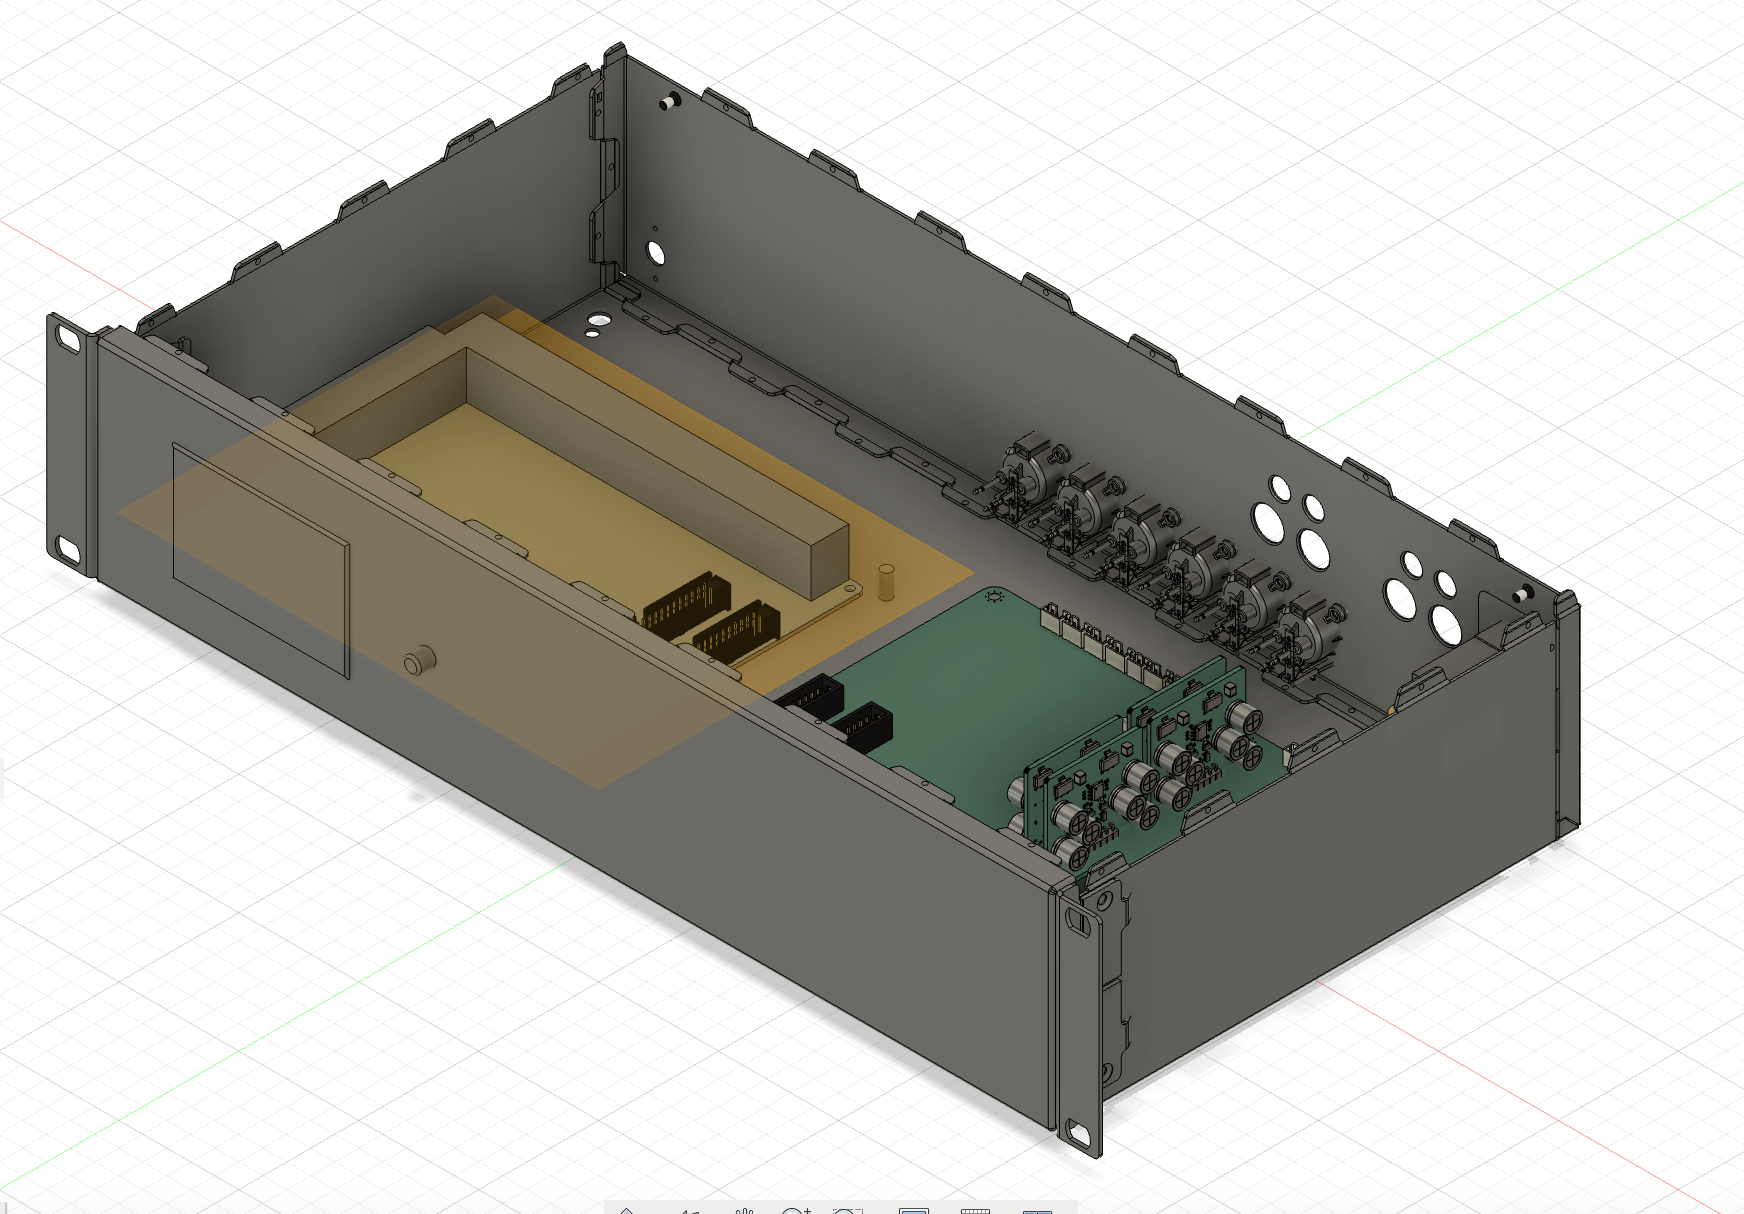
\includegraphics[width=0.8\textwidth]{frontviewcase}
    \caption{Front view of the case}
    \label{fig:frontview}
\end{figure}

\begin{figure}[ht]
    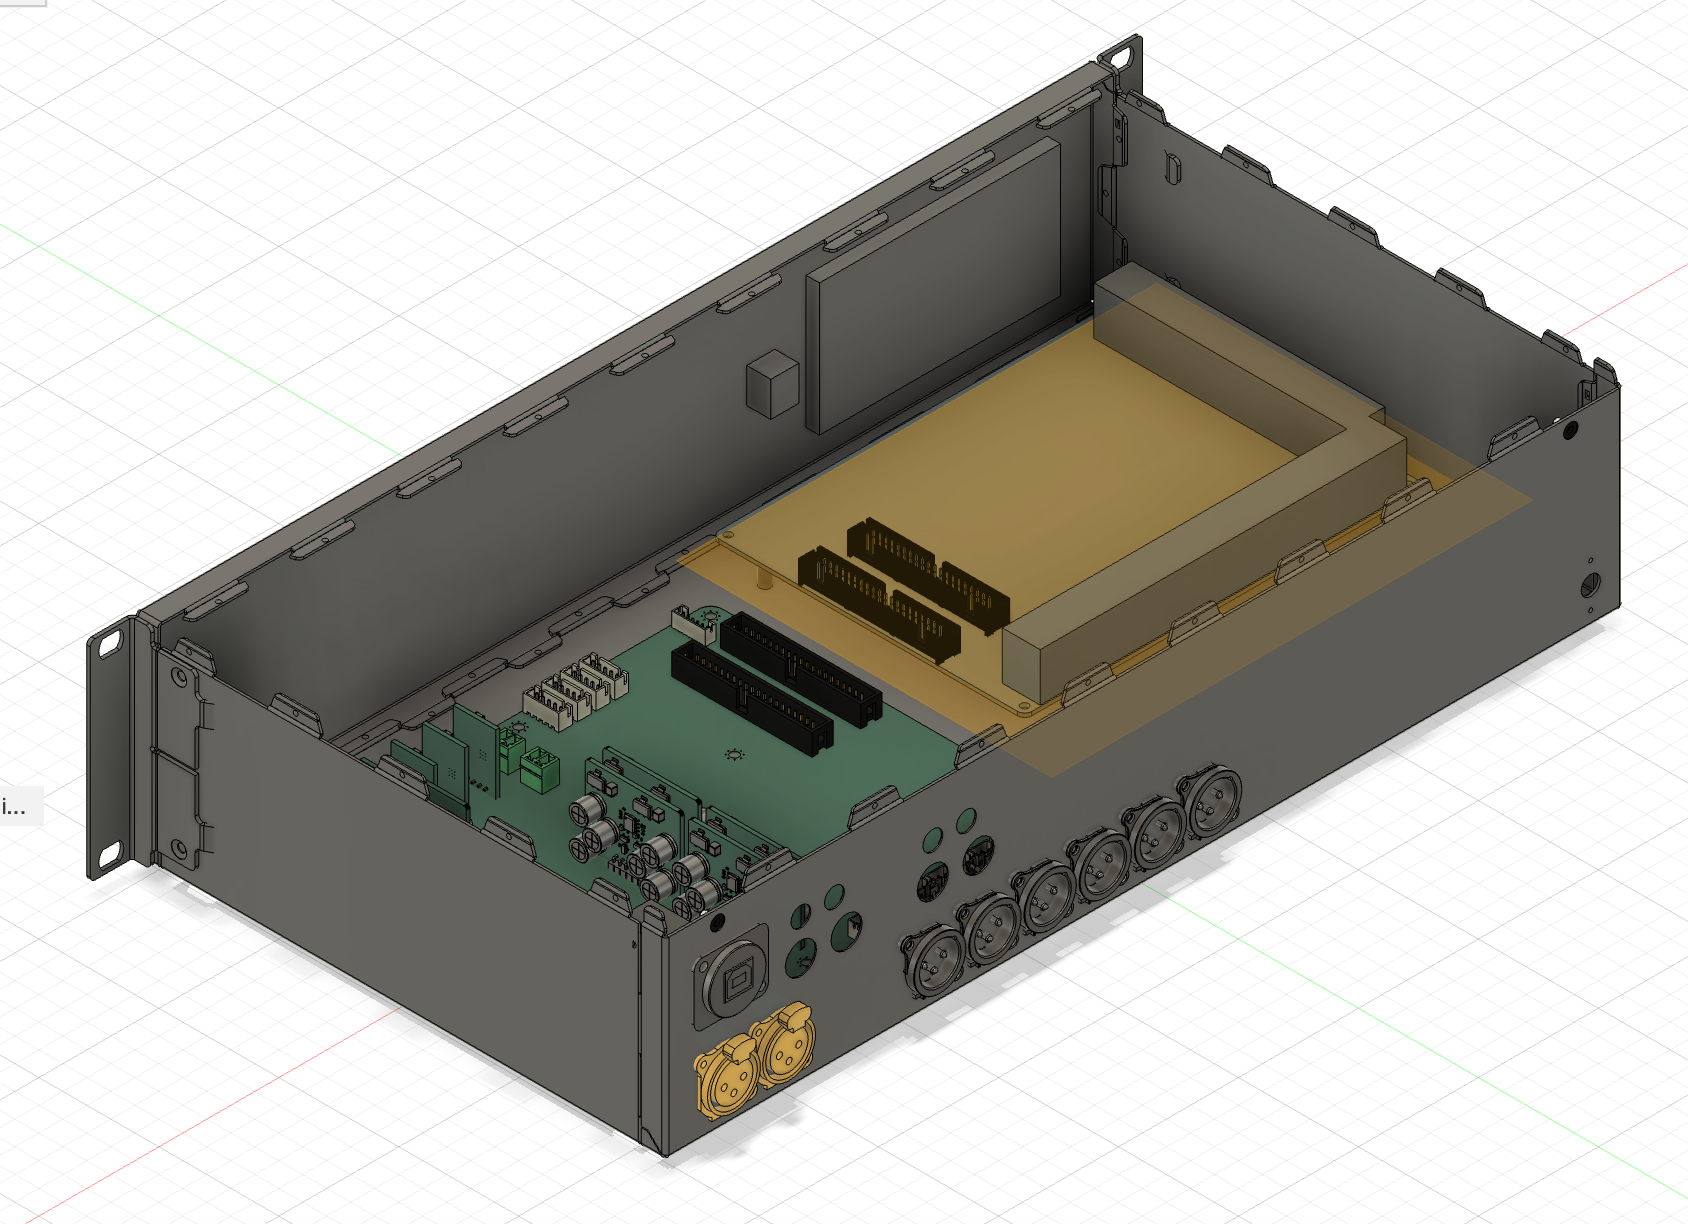
\includegraphics[width=0.8\textwidth]{rearviewcase}
    \caption{Rear view of the case}
    \label{fig:rearview}
\end{figure}

\newpage 